% !TeX program = xelatex
% Options for packages loaded elsewhere
\PassOptionsToPackage{unicode}{hyperref}
\PassOptionsToPackage{hyphens}{url}
\PassOptionsToPackage{dvipsnames,svgnames,x11names}{xcolor}
\PassOptionsToPackage{space}{xeCJK}
%
\documentclass[
  10pt,
  a4paper,
]{article}
\usepackage{amsmath,amssymb}
\usepackage{iftex}
\RequireXeTeX
\usepackage{unicode-math}
\usepackage{xeCJK}
\setmainfont[Path=fonts/,BoldFont=lmroman10-bold.otf,
 ItalicFont=lmroman10-italic.otf,BoldItalicFont=lmroman10-bolditalic.otf]{lmroman10-regular.otf}
\setmonofont[Path=fonts/,BoldFont=lmmono10-regular.otf,
 ItalicFont=lmmono10-italic.otf,BoldItalicFont=lmmono10-italic.otf]{lmmono10-regular.otf}
\setCJKmainfont[Path=fonts/,BoldFont=FandolSong-Bold.otf,
 ItalicFont=FandolKai-Regular.otf]{FandolSong-Regular.otf}
\setCJKmonofont[Path=fonts/]{FandolSong-Regular.otf}
\setCJKsansfont[Path=fonts/,BoldFont=FandolSong-Bold.otf]{FandolSong-Regular.otf}
% Use upquote if available, for straight quotes in verbatim environments
\IfFileExists{upquote.sty}{\usepackage{upquote}}{}
\IfFileExists{microtype.sty}{% use microtype if available
  \usepackage[]{microtype}
  \UseMicrotypeSet[protrusion]{basicmath} % disable protrusion for tt fonts
}{}
\makeatletter
\@ifundefined{KOMAClassName}{% if non-KOMA class
  \IfFileExists{parskip.sty}{%
    \usepackage{parskip}
  }{% else
    \setlength{\parindent}{0pt}
    \setlength{\parskip}{6pt plus 2pt minus 1pt}}
}{% if KOMA class
  \KOMAoptions{parskip=half}}
\makeatother
\usepackage{xcolor}
\usepackage[margin=22mm]{geometry}
\usepackage{color}
\usepackage{fancyvrb}
\newcommand{\VerbBar}{|}
\newcommand{\VERB}{\Verb[commandchars=\\\{\}]}
\DefineVerbatimEnvironment{Highlighting}{Verbatim}{commandchars=\\\{\}}
% Add ',fontsize=\small' for more characters per line
\newenvironment{Shaded}{}{}
\newcommand{\AlertTok}[1]{\textcolor[rgb]{1.00,0.00,0.00}{\textbf{#1}}}
\newcommand{\AnnotationTok}[1]{\textcolor[rgb]{0.38,0.63,0.69}{\textbf{\textit{#1}}}}
\newcommand{\AttributeTok}[1]{\textcolor[rgb]{0.49,0.56,0.16}{#1}}
\newcommand{\BaseNTok}[1]{\textcolor[rgb]{0.25,0.63,0.44}{#1}}
\newcommand{\BuiltInTok}[1]{\textcolor[rgb]{0.00,0.50,0.00}{#1}}
\newcommand{\CharTok}[1]{\textcolor[rgb]{0.25,0.44,0.63}{#1}}
\newcommand{\CommentTok}[1]{\textcolor[rgb]{0.38,0.63,0.69}{\textit{#1}}}
\newcommand{\CommentVarTok}[1]{\textcolor[rgb]{0.38,0.63,0.69}{\textbf{\textit{#1}}}}
\newcommand{\ConstantTok}[1]{\textcolor[rgb]{0.53,0.00,0.00}{#1}}
\newcommand{\ControlFlowTok}[1]{\textcolor[rgb]{0.00,0.44,0.13}{\textbf{#1}}}
\newcommand{\DataTypeTok}[1]{\textcolor[rgb]{0.56,0.13,0.00}{#1}}
\newcommand{\DecValTok}[1]{\textcolor[rgb]{0.25,0.63,0.44}{#1}}
\newcommand{\DocumentationTok}[1]{\textcolor[rgb]{0.73,0.13,0.13}{\textit{#1}}}
\newcommand{\ErrorTok}[1]{\textcolor[rgb]{1.00,0.00,0.00}{\textbf{#1}}}
\newcommand{\ExtensionTok}[1]{#1}
\newcommand{\FloatTok}[1]{\textcolor[rgb]{0.25,0.63,0.44}{#1}}
\newcommand{\FunctionTok}[1]{\textcolor[rgb]{0.02,0.16,0.49}{#1}}
\newcommand{\ImportTok}[1]{\textcolor[rgb]{0.00,0.50,0.00}{\textbf{#1}}}
\newcommand{\InformationTok}[1]{\textcolor[rgb]{0.38,0.63,0.69}{\textbf{\textit{#1}}}}
\newcommand{\KeywordTok}[1]{\textcolor[rgb]{0.00,0.44,0.13}{\textbf{#1}}}
\newcommand{\NormalTok}[1]{#1}
\newcommand{\OperatorTok}[1]{\textcolor[rgb]{0.40,0.40,0.40}{#1}}
\newcommand{\OtherTok}[1]{\textcolor[rgb]{0.00,0.44,0.13}{#1}}
\newcommand{\PreprocessorTok}[1]{\textcolor[rgb]{0.74,0.48,0.00}{#1}}
\newcommand{\RegionMarkerTok}[1]{#1}
\newcommand{\SpecialCharTok}[1]{\textcolor[rgb]{0.25,0.44,0.63}{#1}}
\newcommand{\SpecialStringTok}[1]{\textcolor[rgb]{0.73,0.40,0.53}{#1}}
\newcommand{\StringTok}[1]{\textcolor[rgb]{0.25,0.44,0.63}{#1}}
\newcommand{\VariableTok}[1]{\textcolor[rgb]{0.10,0.09,0.49}{#1}}
\newcommand{\VerbatimStringTok}[1]{\textcolor[rgb]{0.25,0.44,0.63}{#1}}
\newcommand{\WarningTok}[1]{\textcolor[rgb]{0.38,0.63,0.69}{\textbf{\textit{#1}}}}
\usepackage{longtable,booktabs,array}
\usepackage{calc} % for calculating minipage widths
% Correct order of tables after \paragraph or \subparagraph
\usepackage{etoolbox}
\makeatletter
\patchcmd\longtable{\par}{\if@noskipsec\mbox{}\fi\par}{}{}
\makeatother
% Allow footnotes in longtable head/foot
\IfFileExists{footnotehyper.sty}{\usepackage{footnotehyper}}{\usepackage{footnote}}
\makesavenoteenv{longtable}
\usepackage{graphicx}
\makeatletter
\def\maxwidth{\ifdim\Gin@nat@width>\linewidth\linewidth\else\Gin@nat@width\fi}
\def\maxheight{\ifdim\Gin@nat@height>\textheight\textheight\else\Gin@nat@height\fi}
\makeatother
% Scale images if necessary, so that they will not overflow the page
% margins by default, and it is still possible to overwrite the defaults
% using explicit options in \includegraphics[width, height, ...]{}
\setkeys{Gin}{width=\maxwidth,height=\maxheight,keepaspectratio}
% Set default figure placement to htbp
\makeatletter
\def\fps@figure{htbp}
\makeatother
\setlength{\emergencystretch}{3em} % prevent overfull lines
\providecommand{\tightlist}{%
  \setlength{\itemsep}{0pt}\setlength{\parskip}{0pt}}
\setcounter{secnumdepth}{-\maxdimen} % remove section numbering
\ifLuaTeX
\usepackage[bidi=basic]{babel}
\else
\usepackage[bidi=default]{babel}
\fi
\babelprovide[main,import]{chinese}
\ifPDFTeX
\else
\babelfont{rm}[Path=fonts/,BoldFont=lmroman10-bold.otf,ItalicFont=lmroman10-italic.otf,BoldItalicFont=lmroman10-bolditalic.otf]{lmroman10-regular.otf}
\fi
% get rid of language-specific shorthands (see #6817):
\let\LanguageShortHands\languageshorthands
\def\languageshorthands#1{}
\usepackage{float}
\floatplacement{figure}{H}
\newcommand{\serverfigure}[2]{%
\IfFileExists{figures/#1}{\begin{figure}[H]\centering
\includegraphics[width=\linewidth,height=0.72\textheight,keepaspectratio]{figures/#1}
\caption{#2}\end{figure}}{}}
\ifLuaTeX
  \usepackage{selnolig}  % disable illegal ligatures
\fi
\usepackage{bookmark}
\IfFileExists{xurl.sty}{\usepackage{xurl}}{} % add URL line breaks if available
\urlstyle{same}
\hypersetup{
  pdftitle={Lab 1 实验报告},
  pdfauthor={team01},
  pdflang={zh-CN},
  colorlinks=true,
  linkcolor={Maroon},
  filecolor={Maroon},
  citecolor={Blue},
  urlcolor={Blue},
  pdfcreator={LaTeX via pandoc}}

\title{Lab 1 实验报告}
\usepackage{etoolbox}
\makeatletter
\providecommand{\subtitle}[1]{% add subtitle to \maketitle
  \apptocmd{\@title}{\par {\large #1 \par}}{}{}
}
\makeatother
\subtitle{Winograd 卷积、CORDIC 与双缓冲控制器}
\author{team01}
\date{2026 年 11 月 8 日}

\begin{document}
\maketitle

\section{实验概述}\label{ux5b9eux9a8cux6982ux8ff0}

本实验完成一维 Winograd 卷积单元、旋转模式
CORDIC、双缓冲加载与计算控制器，并将 Winograd 扩展为二维 F(2×2,3×3)
卷积单元。设计重点是减少乘法运算、合理安排流水线，以及保证加载和计算之间的数据依赖。

1D Winograd 用四次乘法计算两个相邻卷积点；CORDIC
通过十六级移位加减完成向量旋转；双缓冲控制器利用两个缓冲区实现加载与计算重叠；2D
Winograd 用十六次乘法生成一个 2×2 输出块。各模块保持课程规定的顶层接口。

验证采用课程 Testbench 与独立扩展测试相结合的方法。课程 TB、Makefile
和文件列表保持原样。扩展测试使用直接卷积、浮点旋转参考及多组加载/计算延迟，检查算术结果、流水时序和缓冲区使用。三项课程测试在
VCS 上全部通过，2D 扩展测试在服务器上完成 1200 周期仿真，928
组有效输出均与参考结果一致。

\section{1D Winograd
卷积单元}\label{d-winograd-ux5377ux79efux5355ux5143}

\subsection{接口与计算目标}\label{ux63a5ux53e3ux4e0eux8ba1ux7b97ux76eeux6807}

顶层 \texttt{winograd\_1d} 保留课程全部端口：\texttt{clk,rstn,en}、四个
32 位有符号输入 \texttt{r1\_x} 至 \texttt{r4\_x}、三个 32 位有符号权重
\texttt{r1\_w} 至 \texttt{r3\_w}、两个 32 位有符号结果和
\texttt{vld}。计算等价于：

\[y_0=d_0g_0+d_1g_1+d_2g_2,\quad y_1=d_1g_0+d_2g_1+d_3g_2.\]

结果保留数学整数和的低 32 位，以二补数解释。实现采用 F(2,3)
变换域计算，将直接计算所需的 6 次乘法降为 4 次。

\subsection{定点数与奇数权重}\label{ux5b9aux70b9ux6570ux4e0eux5947ux6570ux6743ux91cd}

直接对权重变换中的分子做整数除以
2，会在奇数权重上丢失半整数信息。因此本设计将权重变换放大 2
倍，延后到输出相加后统一除以 2：

\[b=(d_0-d_2,\ d_1+d_2,\ d_2-d_1,\ d_1-d_3),\]
\[h=(2g_0,\ g_0+g_1+g_2,\ g_0-g_1+g_2,\ 2g_2),\]
\[p_i=b_i h_i,\quad y_0=(p_0+p_1+p_2)/2,\quad y_1=(p_1-p_2-p_3)/2.\]

分子在精确整数运算下必为偶数，因此输出选择第 32 至第 1 位，等价于精确除
2 后保留低 32 位。负数同样成立，不存在提前截断带来的舍入误差。

\begin{longtable}[]{@{}lrl@{}}
\toprule\noalign{}
信号 & 有符号位宽 & 目的 \\
\midrule\noalign{}
\endhead
\bottomrule\noalign{}
\endlastfoot
输入特征及原权重 & 32 & 保持课程接口 \\
输入变换 b & 33 & 两个 32 位数加减前符号扩展 \\
放大的权重变换 h & 34 & 三项加减或乘 2，不丢高位 \\
四个乘积 p & 67 & 完整容纳 33×34 位乘法 \\
输出求和 & 69 & 为三项加减保留余量 \\
输出 & 32 & 取求和结果 \texttt{{[}32:1{]}} \\
\end{longtable}

\texttt{input\_transform.v}、\texttt{weight\_transform.v}、\texttt{output\_transform.v}
为组合逻辑；\texttt{winograd\_1d.v} 组织三级寄存流水线。

\subsection{时序与复位}\label{ux65f6ux5e8fux4e0eux590dux4f4d}

\begin{longtable}[]{@{}lll@{}}
\toprule\noalign{}
沿 & 工作 & 有效位 \\
\midrule\noalign{}
\endhead
\bottomrule\noalign{}
\endlastfoot
第 1 沿 n & 接收输入，寄存输入/权重变换 & \texttt{v1\ ←\ en} \\
第 2 沿 n+1 & 寄存四个变换域乘积 & \texttt{v2\ ←\ v1} \\
第 3 沿 n+2 & 寄存输出变换结果 & \texttt{vld\ ←\ v2} \\
\end{longtable}

以 25ns 接收第一组输入为例，其结果在 45ns
上升沿后有效。每拍可接收一组输入；\texttt{en=0}
形成空泡，结果总线可继续变化，只有 \texttt{vld=1}
时表示有效。低有效异步复位清除全部流水寄存器、结果和有效位，丢弃在途输入。

\begin{figure}
\centering
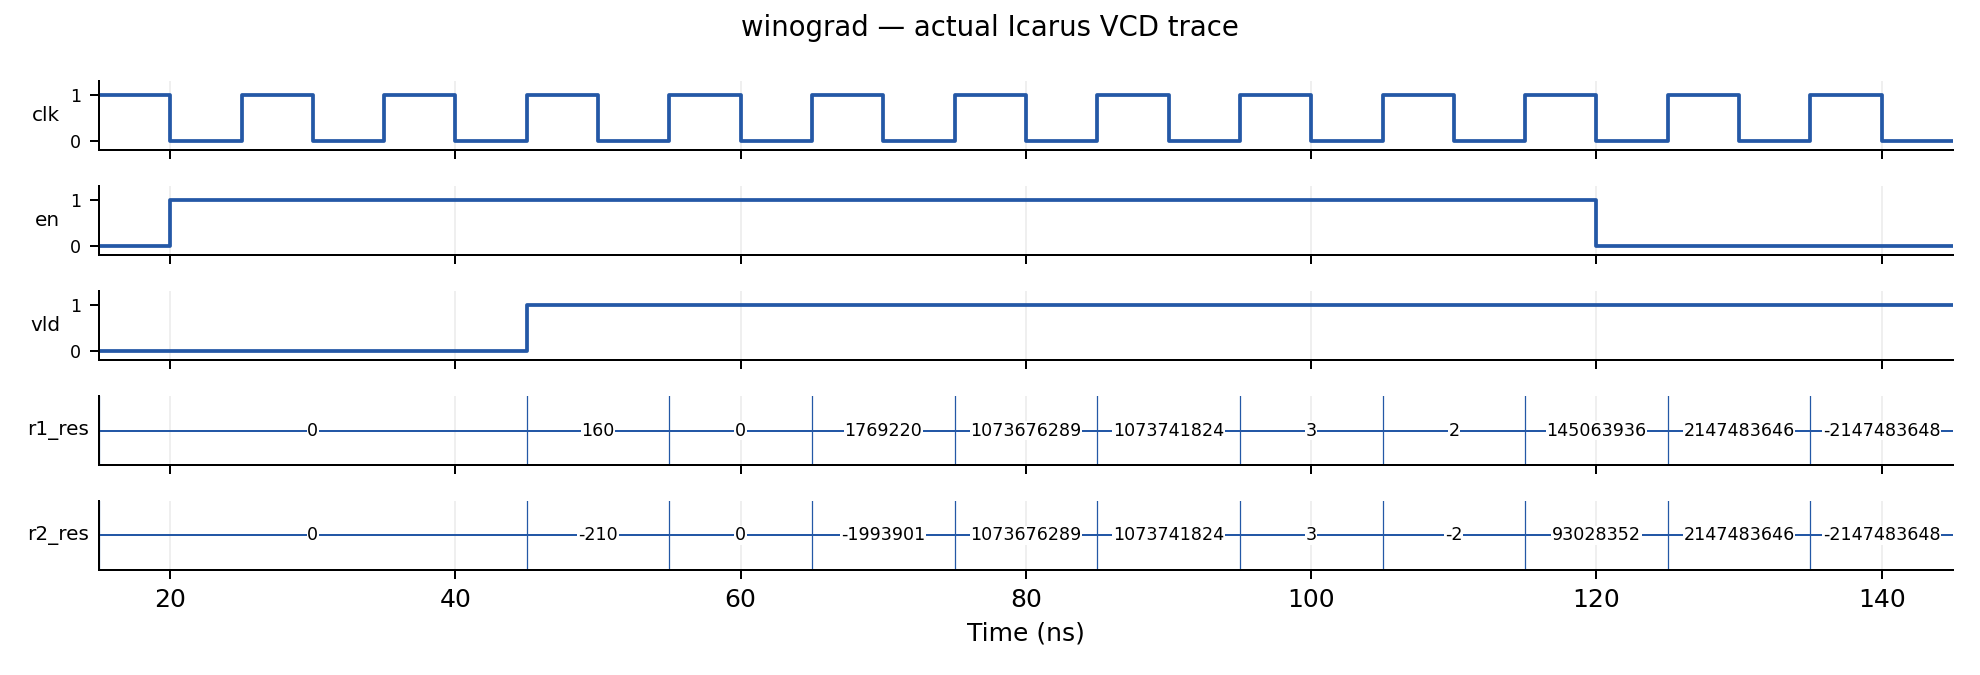
\includegraphics{figures/winograd.png}
\caption{本地 Icarus VCD 绘图：1D Winograd；25ns 采样的第一组结果在 45ns
后输出，后续结果逐拍出现。}
\end{figure}

\subsection{运算等价性与位宽分析}\label{ux8fd0ux7b97ux7b49ux4ef7ux6027ux4e0eux4f4dux5bbdux5206ux6790}

将前述变换代入第一路输出分子：

\[2(d_0-d_2)g_0+(d_1+d_2)(g_0+g_1+g_2)+(d_2-d_1)(g_0-g_1+g_2)\]
\[=2(d_0g_0+d_1g_1+d_2g_2).\]

第二路同理得到 \(2(d_1g_0+d_2g_1+d_3g_2)\)。因此，输出统一除 2
可精确恢复直接卷积结果。计算采用题目规定的滑动点积形式，权重顺序与输入窗口一致。

输入差和最多需要 33 位；三个 32 位权重相加或相减需要 34 位；33×34
位乘法用 67 位保存，输出求和用 69 位。符号扩展在运算之前完成。最终取
{[}32:1{]}，等于精确除 2 后取低 32 位。中间不发生会影响该结果的截断。

\section{CORDIC 设计}\label{cordic-ux8bbeux8ba1}

\subsection{角度与全象限变换}\label{ux89d2ux5ea6ux4e0eux5168ux8c61ux9650ux53d8ux6362}

顶层 \texttt{cordic} 按课程端口顺序保留
\texttt{clock,xstart,ystart,zangle,xout,yout,done}。\texttt{zangle}
按无符号 32 位圆周编码解释，一周对应 \(2^{32}\)；90°、180°、270° 分别为
\texttt{0x40000000}、\texttt{0x80000000}、\texttt{0xC0000000}。

当最高两位为 \texttt{01} 或 \texttt{10}，先将初始向量取反，同时角度减去
180°。其余角度直接按有符号 32 位剩余角度解释。这样进入 CORDIC 的角度位于
−90° 至 +90° 范围内，覆盖全圆，包括边界 90°、180°、270°、359°。

\subsection{16 级旋转流水线}\label{ux7ea7ux65cbux8f6cux6d41ux6c34ux7ebf}

每一级迭代 i 使用当前剩余角度的符号确定旋转方向：

\[x_{i+1}=x_i-\sigma_i(y_i\mathbin{\ggg}i),\]
\[y_{i+1}=y_i+\sigma_i(x_i\mathbin{\ggg}i),\]
\[z_{i+1}=z_i-\sigma_i\arctan(2^{-i}).\]

其中 \(\sigma_i=1\)（当 \(z_i\geq0\)），否则为
−1；\texttt{\textgreater{}\textgreater{}\textgreater{}}
是算术右移。查表值将反正切角度按圆周编码四舍五入为整数常量，RTL 中不使用
real 或运行时三角函数。16 次迭代均由加减法、移位及常量构成，无乘法器。

内部 x/y 为 34 位有符号数，输入左移 16
位保留小数位，另有符号及幅度余量。输出加半个整数单位后算术右移 16
位，舍入后截取 16
位。无饱和逻辑；任意过大输入向量可能溢出，但课程规定幅度不溢出。

迭代增益约为 1.646760258。课程 TB 已将 \texttt{xstart} 设置为约
\texttt{32000/1.64676=19432}、\texttt{ystart=0}，因此模块不再重复做增益补偿，输出约为
\texttt{32000*cos(theta)} 和 \texttt{32000*sin(theta)}。

输入至输出有 16 个寄存级。输入稳定保持至少 16 个上升沿后输出稳定；课程
4ns 时钟下 70ns 后读取满足要求。可每拍接收不同向量，但 \texttt{done}
不用于输入握手。接口没有 reset/start，\texttt{done} 用初始化为零的 16
位有效移位寄存器，在填满后持续为
1，表示流水线有数据；它不是单周期任务完成脉冲。此初始化适用于本次仿真及支持寄存器初始化的
FPGA；

\begin{figure}
\centering
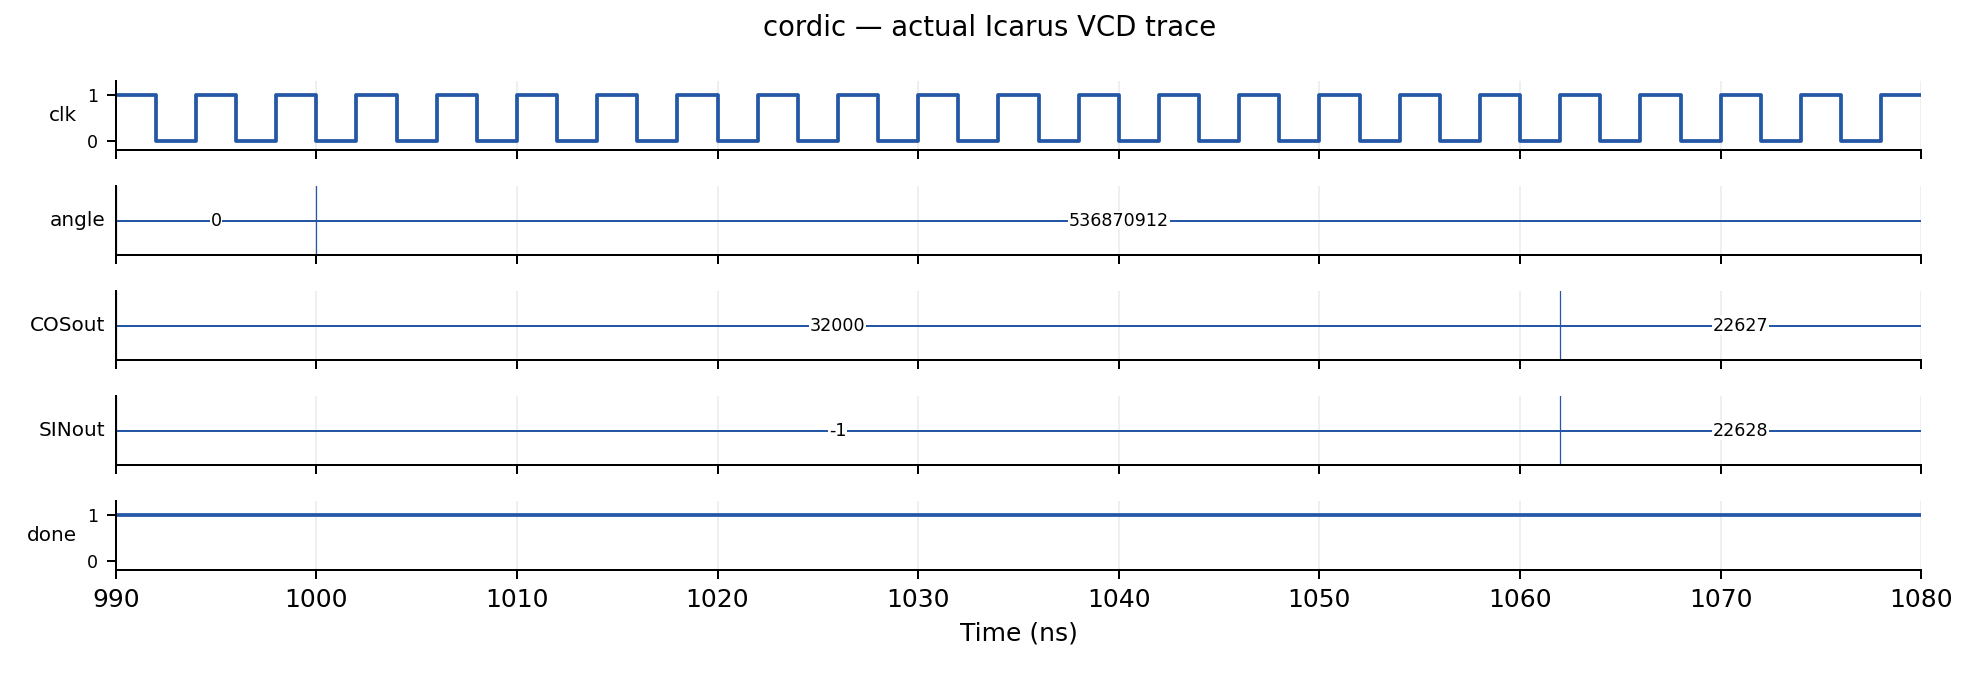
\includegraphics{figures/cordic.png}
\caption{本地 Icarus VCD 绘图：CORDIC；1000ns 更新到 45°，16
个上升沿后输出为 22627、22628，满足误差上限。}
\end{figure}

\subsection{收敛范围与误差分析}\label{ux6536ux655bux8303ux56f4ux4e0eux8befux5deeux5206ux6790}

象限预处理将角度映射到 −90° 至
+90°，落入旋转模式收敛区间；向量取反配合角度减 180° 保持最终旋转一致。16
级增益
\(K=\prod_{i=0}^{15}\sqrt{1+2^{-2i}}\approx1.646760258\)，课程输入已按该增益预补偿。

末级角度步长约为 \(\arctan(2^{-15})\approx3.05\times10^{-5}\) 弧度，对
32000
幅度的坐标影响约为一个整数单位量级，另有角度表量化、移位截断和最终舍入误差。课程要求两路输出的绝对误差均不超过
8，独立扩展测试实测最大误差为 1。

34 位内部表示含 16 位小数，对 16 位输入经 CORDIC
增益后的内部坐标留有幅度余量。最终 16
位端口无饱和功能，任意大初始向量可能输出回绕；课程规定的输入幅度处于有效范围。接口没有
reset/start，done 用于指示流水线已经填满。

\section{双缓冲 FSM 设计}\label{ux53ccux7f13ux51b2-fsm-ux8bbeux8ba1}

\subsection{状态组织与依赖}\label{ux72b6ux6001ux7ec4ux7ec7ux4e0eux4f9dux8d56}

顶层 \texttt{double\_buffer\_ctrl}
保留课程全部端口、方向和位宽。采用分解式 FSM：全局
\texttt{busy}（IDLE/RUN）、加载器 \texttt{loading}（FREE/WAIT）、计算器
\texttt{computing}（FREE/WAIT），以及两个缓冲区的 \texttt{occupied} 和
\texttt{ready} 标记。\texttt{next\_load} 和 \texttt{next\_compute} 各为
2 位，依次取 0、1、2，完成后为 3。

缓冲区映射固定为 tile
编号最低位：tile0→buffer0、tile1→buffer1、tile2→buffer0。请求发出即占用缓冲区，加载完成才置
ready；计算结束才释放 occupied。即使加载器空闲，也不能提前将 tile2
放进仍保存 tile0 的 buffer0。

\begin{longtable}[]{@{}
  >{\raggedright\arraybackslash}p{(\columnwidth - 4\tabcolsep) * \real{0.3333}}
  >{\raggedright\arraybackslash}p{(\columnwidth - 4\tabcolsep) * \real{0.3333}}
  >{\raggedright\arraybackslash}p{(\columnwidth - 4\tabcolsep) * \real{0.3333}}@{}}
\toprule\noalign{}
\begin{minipage}[b]{\linewidth}\raggedright
状态/事件
\end{minipage} & \begin{minipage}[b]{\linewidth}\raggedright
条件
\end{minipage} & \begin{minipage}[b]{\linewidth}\raggedright
动作及下一状态
\end{minipage} \\
\midrule\noalign{}
\endhead
\bottomrule\noalign{}
\endlastfoot
IDLE + start & 当前不忙 & 清计数和缓冲状态，进入 RUN \\
RUN + start & 当前忙 & 忽略 start，不重启、不排队 \\
加载器 FREE & 尚有 tile，目标 buffer 空闲，上拍 req 已低 & 发出一拍
load\_req，标记占用，进入 WAIT \\
加载器 WAIT + load\_done & 有在途加载 & 目标 buffer 置 ready，回 FREE \\
计算器 FREE & 下一个顺序 tile 已 ready，上拍 req 已低 & 发出一拍
compute\_req，进入 WAIT \\
计算器 WAIT + compute\_done & tile0 或 tile1 & 释放对应 buffer，回
FREE \\
计算器 WAIT + compute\_done & tile2 & 清 busy，产生一拍 done，进入
IDLE \\
任意状态 + rstn=0 & 低有效异步复位 & 中止任务并清除所有输出和状态 \\
\end{longtable}

组合下一状态逻辑先消费本沿完成事件，再判断可以发出的请求。因此可以在接收
tile0 加载完成后，并行安排加载 tile1 和计算 tile0；在接收 tile0
计算完成后，并行安排加载 tile2 和计算 tile1（若 tile1 已
ready）。不会为等待另一引擎而阻塞独立工作。

为满足请求必须是独立单周期脉冲的要求，上一拍请求为高时不连续发出同类请求；这只是脉冲分隔，不是对另一引擎的等待。外部
done 必须对应已发出的请求，且不得与请求同周期完成，符合课程协议。

\subsection{关键重叠波形}\label{ux5173ux952eux91cdux53e0ux6ce2ux5f62}

\begin{figure}
\centering
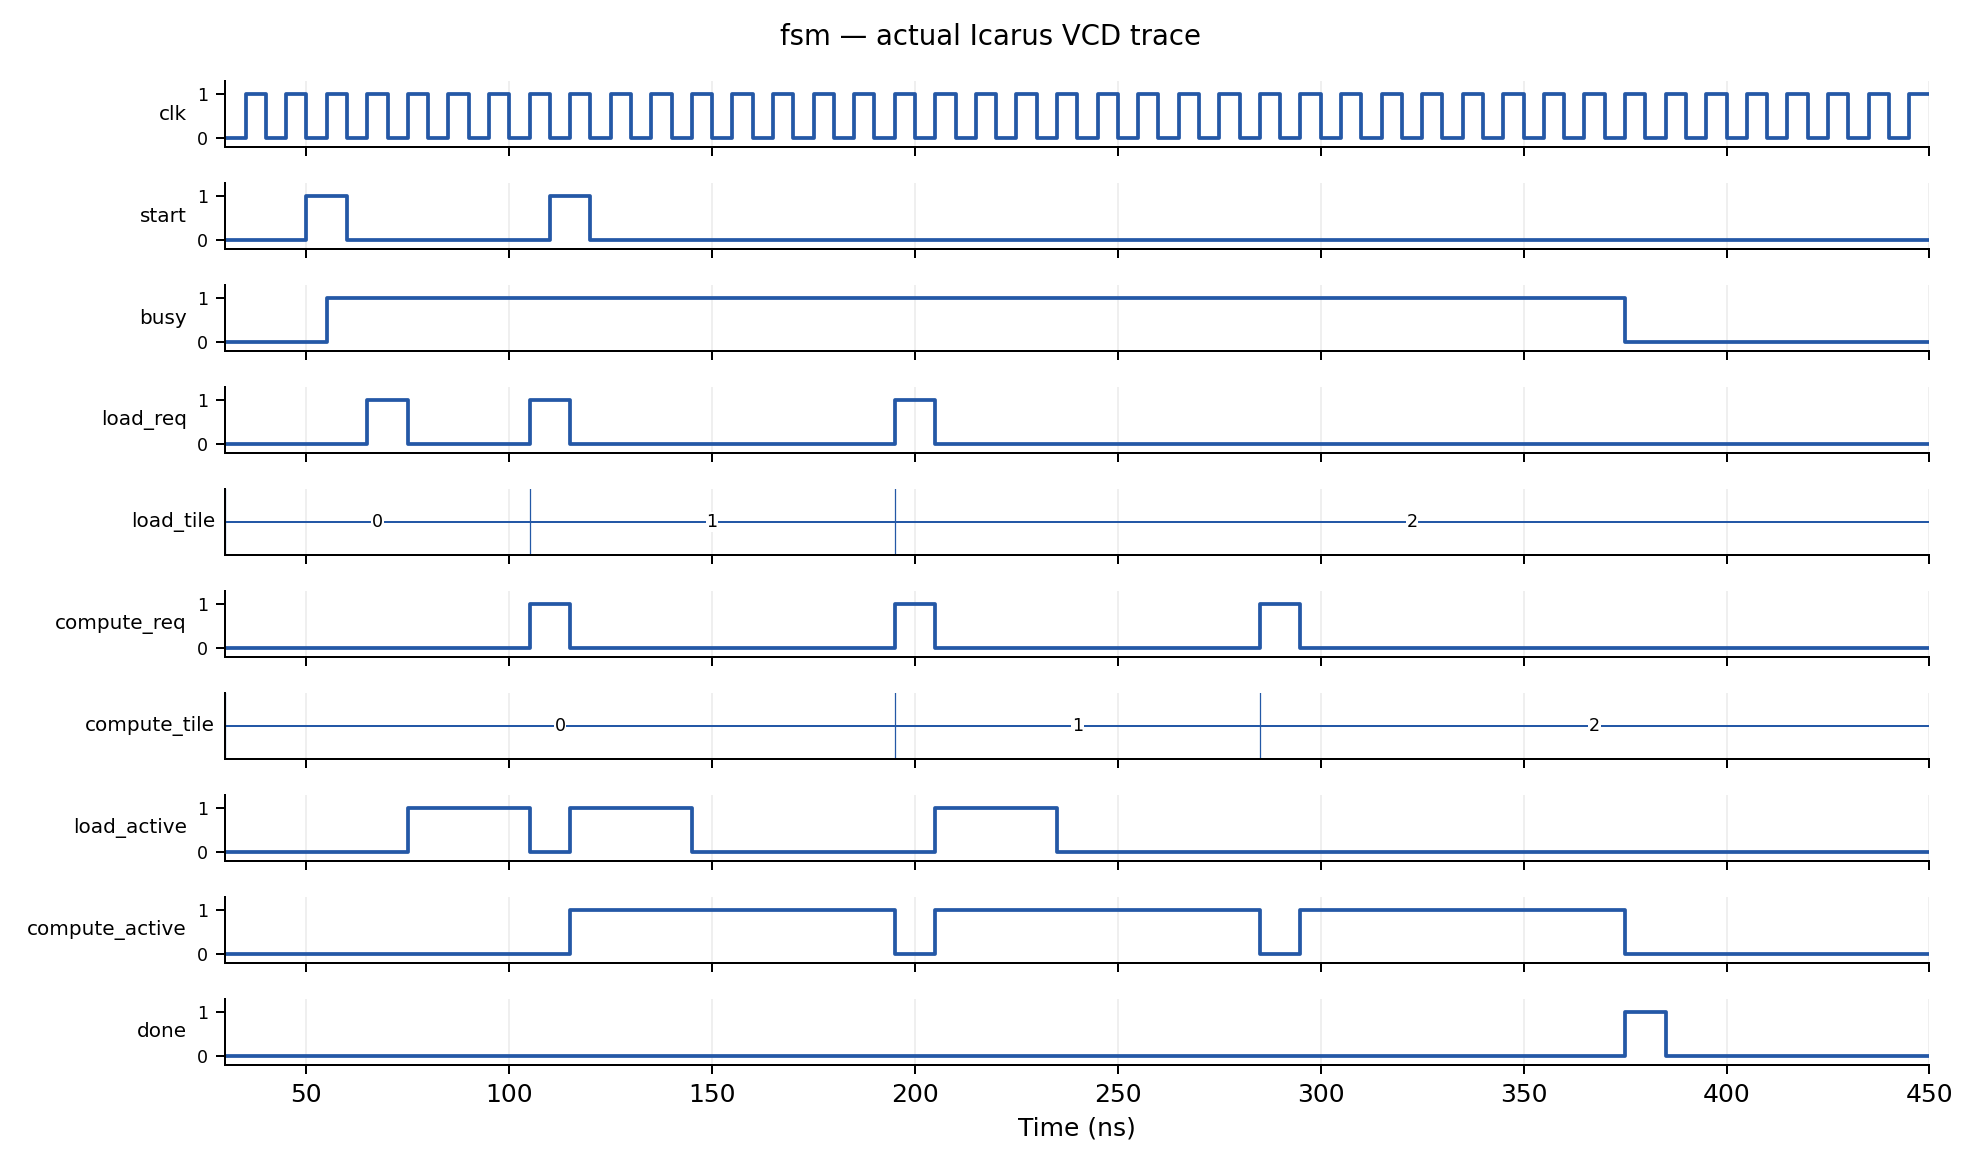
\includegraphics{figures/fsm.png}
\caption{本地 Icarus VCD 绘图：FSM；tile1 加载与 tile0 计算重叠，tile2
加载与 tile1 计算重叠；忙碌中的第二次 start 被忽略。}
\end{figure}

图中 105ns 同时发出 tile1 的加载请求和 tile0 的计算请求；195ns 发出
tile2 的加载请求和 tile1 的计算请求。两个阶段使用不同缓冲区。约 375ns
收到最后计算完成后，done 为单周期高电平，busy 返回低电平。

\subsection{状态约束与任务完成条件}\label{ux72b6ux6001ux7ea6ux675fux4e0eux4efbux52a1ux5b8cux6210ux6761ux4ef6}

正确性可按时钟沿归纳理解：复位时两个 buffer 均空闲；只有空闲目标 buffer
才允许加载，请求发出立即占用；只有加载完成才设 ready；计算请求只选择
next\_compute 指定的 ready
buffer；仅计算完成才释放占用。因此从初始状态出发，不会对未加载 tile
发计算请求，也不会覆盖未计算完的数据。

next\_load、next\_compute 单调从 0 走到 3，每次请求只增加一次，保证每个
tile
一次加载、一次计算，计算顺序固定。两个引擎的在途标志防止同一引擎同时接受两个任务。tile2
的 buffer0 复用受 occupied 限制。只有 tile2 的计算完成才产生一拍
done，busy 期间忽略 start，复位丢弃在途任务。

控制器遵循课程握手协议：完成脉冲对应已发出的请求，且晚于请求周期。在加载器和计算器均正常返回完成信号的条件下，三个
tile 依次完成，控制器回到空闲状态。

\section{2D Winograd
卷积单元（Bonus）}\label{d-winograd-ux5377ux79efux5355ux5143bonus}

实现 F(2×2,3×3)，输入 4×4、权重 3×3、输出 2×2，顶层名为
\texttt{winograd\_2d}。接口为
\texttt{clk}、\texttt{rstn}、\texttt{en}、\texttt{x\_flat{[}511:0{]}}、\texttt{w\_flat{[}287:0{]}}、\texttt{res\_flat{[}127:0{]}}、\texttt{vld}。沿用
1D 的第 1 沿采样、第 3 沿输出和每拍吞吐规则。

打包采用行优先顺序，第 0 个元素位于最低 32 位，即第 i 个元素对应
\texttt{{[}32*i\ +:\ 32{]}}。输入、权重和输出遵循同一约定。

使用与 1D 相同的 B、G、A 变换矩阵，先按行、再按列分离计算：

\[V=B^TdB,\quad U=(2G)w(2G)^T,\quad Y=A^T(U\odot V)A/4.\]

权重变换扩大 4 倍，输出求和后统一除 4。仅有 16
次变换域乘法，而四个输出逐个直接卷积需要 36 次乘法。输入变换 34
位、权重变换 36 位、乘积 70 位、输出求和 74 位，最终取
\texttt{{[}33:2{]}} 实现除 4 后低 32
位输出。中间结果不提前丢弃小数或有效整数位。

独立 Testbench 由脚本生成，Golden Model 使用 Python
任意精度整数直接做四个 3×3 卷积，再截取低 32 位；与 RTL 的变换算法独立。

\subsection{二维变换的等价性}\label{ux4e8cux7ef4ux53d8ux6362ux7684ux7b49ux4ef7ux6027}

一维恒等式分别作用于行和列，即得到
\(A^T[(GwG^T)\odot(B^TdB)]A\)。实现将两次权重变换各扩大 2
倍，因此整体扩大 4 倍；最后统一除
4。精确整数运算下每个输出分子均是对应直接卷积和的 4 倍。

输入二维变换最多为四个原数的带符号和，34
位足够。权重变换的最大绝对系数和为 9，36 位足够容纳完整 32
位输入范围；34×36 位乘积保存为 70 位，输出中最多九项乘积组合用 74
位留出余量。最终 {[}33:2{]} 等于除 4 后取低 32 位。乘以常数 2
的表达式可化为移位，不计为一般数据乘法器。

行优先打包且元素 0 在最低 32
位是本实现明确使用的约定；测试采用同一约定。各输入矩阵及输出矩阵均采用这一打包约定。

\section{运算效率与硬件开销}\label{ux8fd0ux7b97ux6548ux7387ux4e0eux786cux4ef6ux5f00ux9500}

\begin{longtable}[]{@{}
  >{\raggedright\arraybackslash}p{(\columnwidth - 4\tabcolsep) * \real{0.3333}}
  >{\raggedright\arraybackslash}p{(\columnwidth - 4\tabcolsep) * \real{0.3333}}
  >{\raggedright\arraybackslash}p{(\columnwidth - 4\tabcolsep) * \real{0.3333}}@{}}
\toprule\noalign{}
\begin{minipage}[b]{\linewidth}\raggedright
项目
\end{minipage} & \begin{minipage}[b]{\linewidth}\raggedright
运算量或资源结构
\end{minipage} & \begin{minipage}[b]{\linewidth}\raggedright
延迟与吞吐
\end{minipage} \\
\midrule\noalign{}
\endhead
\bottomrule\noalign{}
\endlastfoot
1D & 4 次一般乘法，直接算法为 6 次，减少约 33.3\% & 第 1 沿采样、第 3
沿输出；可每拍接收一组 \\
2D & 16 次一般乘法，直接算法为 36 次，减少约 55.6\% &
同样三级流水；每拍可产生一个 2×2 块 \\
CORDIC & 16 级展开，每级坐标加减和角度加减，移位量为常数 & 每组经过 16
个寄存级；结构可每拍接收一组 \\
FSM & 少量状态、计数器和两个 buffer 的占用/就绪位 & 不同 buffer
的加载与计算可以重叠 \\
\end{longtable}

Winograd 的第 1 沿为采样沿，结果在两周期后的第 3 沿输出。CORDIC
采用逐级寄存结构，具备每周期接收一组输入的结构条件；本次测试按课程要求保持输入稳定，检查十六级迭代后的结果。

Winograd 通过增加变换加减法来减少乘法次数。为覆盖完整的 32
位输入范围，本实现使用较宽的乘法器和流水寄存器，硬件开销由乘法、变换逻辑和寄存器共同构成。特别是
2D 行列组合变换集中在寄存级之间，可能形成较长加法链。CORDIC
的展开结构用更多硬件换吞吐；复用单个迭代单元会省资源但降低吞吐。

若忽略控制开销，加载时长为 L、计算时长为 C，三个 tile 完全串行为
\(3(L+C)\)；理想重叠可接近 \(L+C+2\max(L,C)\)。当 L=C 时，由 6L 降到约
4L，理想加速约 1.5
倍。实际执行时间还包含请求/完成采样及脉冲间隔产生的控制开销。

本节以算法运算量、流水级数和控制重叠分析效率；具体面积、时钟频率和功耗需通过综合与实现工具进一步测量。

\section{验证方案}\label{ux9a8cux8bc1ux65b9ux6848}

\subsection{课程 Testbench}\label{ux8bfeux7a0b-testbench}

1D 的 10 组测试使用直接卷积 Golden Model，检查低 32 位结果、有效位和
X/Z，要求零误差。CORDIC 的 10 个角度为
45°、15°、30°、60°、75°、90°、180°、270°、359°、57°，参考为
32000*cos/sin，两个输出各允许误差 8，含 X/Z 判失败。FSM
三项分别覆盖加载较快、计算较快和任务中复位，并检查 tile
顺序、缓冲区复用、资源占用、重叠和忙碌时 start。

每次比较满足数值及控制条件后，TB 输出 PASS；全部用例通过后输出 ALL
PASS。

\subsection{自编 1D/2D
流水测试}\label{ux81eaux7f16-1d2d-ux6d41ux6c34ux6d4bux8bd5}

脚本 scripts/extended.py 使用固定种子 20261101。每个元素有 35\% 概率从
0、1、−1、最大正数和最小负数中选取，其余取随机 32 位数并按有符号解释。1D
共 2400 周期，2D 共 1200 周期；独立随机 en 约 80\%
有效，形成连续输入与空泡。每 211
周期安排两周期低复位，末尾四周期停止输入以排空流水线。

Python 任意精度整数计算普通直接卷积，最后逐输出保留低 32
位；参考算法不使用 RTL 的 Winograd
变换，从而避免参考模型与被测设计共享同一变换错误。2D
计算四个窗口，各九项乘积相加，权重不翻转，然后以低位优先行主序打包。

TB 在下降沿读向量并设置输入，在上升沿将 en 和参考结果移入独立队列，等待
1ns 后比较。vld 每周期必须等于延迟后的 a2；vld 有效时 y 必须与 q2
逐位相等。复位时有效队列、参考队列清零，并要求输出清零。使用 !==
能将有效结果中的 X/Z 判为失败。无效周期不检查无意义的结果数据。

\begin{longtable}[]{@{}
  >{\raggedright\arraybackslash}p{(\columnwidth - 4\tabcolsep) * \real{0.3333}}
  >{\raggedright\arraybackslash}p{(\columnwidth - 4\tabcolsep) * \real{0.3333}}
  >{\raggedright\arraybackslash}p{(\columnwidth - 4\tabcolsep) * \real{0.3333}}@{}}
\toprule\noalign{}
\begin{minipage}[b]{\linewidth}\raggedright
风险
\end{minipage} & \begin{minipage}[b]{\linewidth}\raggedright
用例与检查
\end{minipage} & \begin{minipage}[b]{\linewidth}\raggedright
为什么需要
\end{minipage} \\
\midrule\noalign{}
\endhead
\bottomrule\noalign{}
\endlastfoot
有符号扩展错误 & 正负随机值、极值，逐位比较 & 暴露中间位宽和 signed
传播问题 \\
奇数权重提前除法 & 随机奇数权重，直接卷积参考 &
发现半整数信息过早丢失 \\
高位溢出处理错误 & 极值及大幅随机数，低 32 位比较 &
验证回绕而非饱和行为 \\
行列或打包顺序错误 & 非对称随机矩阵及四个输出整体比较 &
避免对称样例掩盖转置错误 \\
数据/有效位错拍 & 连续输入、空泡、独立队列 & 检查吞吐及第 3
沿对应关系 \\
在途复位失效 & 周期性复位、清空参考队列 & 发现旧结果在复位后泄出 \\
最后几组漏检 & 停止输入并排空流水线 & 覆盖尾部仍在处理的输入 \\
\end{longtable}

1D 实测 1861 组有效输出全部一致；2D 实测 928
组有效输出全部一致，即比较了 3712 个 32
位卷积结果。每组包含四个输出；1200
周期包括有效输入、复位、空泡和末尾排空。

上述用例分别针对算术精度、矩阵索引、流水线对齐及复位行为。算法等价推导给出计算依据，位宽分析保证中间结果完整，独立参考比较则检查
RTL 对这些规则的落实情况，形成从算法到实现的验证过程。

\subsection{自编 CORDIC 与 FSM
扩展测试}\label{ux81eaux7f16-cordic-ux4e0e-fsm-ux6269ux5c55ux6d4bux8bd5}

CORDIC 对全圆每隔 0.25° 扫描，共 1440 个角度，另加 128
组随机角度和安全范围内的正负初始向量（包含非零 y）。共 1568
组。参考以实际角度编码和输入向量计算理想旋转，乘以 16
级理论增益；每组保持 16 个上升沿后检查两路误差、X/Z 和 done。最大误差为
1。这与课程 TB 固定 32000
幅度参考不同，二者分别运行，未替换课程参考或放宽容差。

FSM 扩展使用加载/计算延迟集合 \{1,2,3,5,8,13\} 的笛卡尔积，共 36
组，并运行任务中复位。延迟从很短到较长，包含两者相等、加载快和计算快三种关系，复用原课程
scoreboard
的全部断言。这些组合覆盖了两类引擎相互等待和并行工作的典型情况。

\section{仿真结果与分析}\label{ux4effux771fux7ed3ux679cux4e0eux5206ux6790}

\subsection{验证环境与结果汇总}\label{ux9a8cux8bc1ux73afux5883ux4e0eux7ed3ux679cux6c47ux603b}

课程服务器使用 VCS Q-2020.03-SP2-7 Full64，波形通过 Verdi 查看，FSDB
Dumper 版本为 Verdi-R-2020.12-SP1。本地扩展验证使用 Icarus Verilog
12.0。服务器结果依据终端运行记录及 Verdi
截图整理；本地结果依据仿真日志统计。FSM 于 2026 年 11 月 8
日在独立目录中完成复验，采用不启用 \texttt{-debug\_access+r} 的 VCS
配置。此次编译日志未出现段错误，运行结果为三项 PASS 和 ALL PASS；RTL
与课程 TB 保持原验证版本。

\begin{longtable}[]{@{}lll@{}}
\toprule\noalign{}
测试项目 & 环境 & 结果 \\
\midrule\noalign{}
\endhead
\bottomrule\noalign{}
\endlastfoot
1D Winograd 课程 TB & VCS & 10/10 通过，误差为 0 \\
CORDIC 课程 TB & VCS & 10/10 通过，截图中最大绝对误差为 1 \\
FSM 课程 TB & VCS（不启用调试访问） & 两组延迟和运行中复位均通过 \\
1D 扩展测试 & Icarus & 2400 周期，1861 组有效输出全部一致 \\
2D 扩展测试 & VCS、Icarus & 1200 周期，928 组有效输出全部一致 \\
CORDIC 扩展测试 & Icarus & 1568 组向量通过，最大绝对误差为 1 \\
FSM 扩展测试 & Icarus & 36 组延迟组合和运行中复位均通过 \\
\end{longtable}

三项课程测试的服务器汇总为：

\begin{Shaded}
\begin{Highlighting}[]
\NormalTok{winograd: 10 PASS; ALL PASS}
\NormalTok{cordic: 10 PASS; ALL PASS}
\NormalTok{fsm: 3 PASS; ALL PASS}
\end{Highlighting}
\end{Shaded}

\serverfigure{server-summary.png}{三项课程测试的服务器运行结果。}

\subsection{1D
Winograd：结果与有效位对齐}\label{d-winogradux7ed3ux679cux4e0eux6709ux6548ux4f4dux5bf9ux9f50}

第一组输入在 25ns 被采样，45ns 上升沿后输出为 160 和 −210，TB 在 46ns
完成比较。这一过程符合``第 1 沿采样、第 3
沿输出''的时序要求。随后连续十组结果按顺序输出；en 在 120ns
降低后，流水线继续输出在途结果，直到最后一组完成后 vld 才变低。

Verdi 中 passed 最终显示十六进制 a，即十进制 10，failed 保持 0。第一组
r1\_res=0xa0 对应 160，r2\_res=0xffffff2e 按二补数解释为
−210。边界用例的输出包括 2147483646 和 −2147483648，与 Golden Model 的低
32 位结果一致。数值比较和有效位检查共同验证了整数计算及流水线对齐。

\serverfigure{server-winograd-log.png}{1D Winograd 课程测试结果。}
\serverfigure{server-winograd-wave.png}{1D Winograd 的服务器 Verdi 波形。}

\subsection{CORDIC：全象限旋转结果}\label{cordicux5168ux8c61ux9650ux65cbux8f6cux7ed3ux679c}

课程测试覆盖第一象限内的多个角度，以及 90°、180°、270° 和接近一周的
359°。代表性结果如下：

\begin{longtable}[]{@{}llll@{}}
\toprule\noalign{}
角度 & 参考值 (cos, sin) & 输出 (xout, yout) & 两路绝对误差 \\
\midrule\noalign{}
\endhead
\bottomrule\noalign{}
\endlastfoot
45° & (22627, 22627) & (22627, 22628) & (0, 1) \\
90° & (0, 32000) & (1, 32000) & (1, 0) \\
180° & (−32000, 0) & (−32000, 1) & (0, 1) \\
270° & (0, −32000) & (−1, −32000) & (1, 0) \\
359° & (31995, −558) & (31995, −559) & (0, 1) \\
\end{longtable}

Verdi 波形中 Xin=0x4be8，即
19432，Yin=0；角度编码依次变化，输出经过流水线延迟后稳定。输出 0x8300
按有符号 16 位解释为 −32000。done 在流水线填满后持续为高，passed 最终为
10，failed 为 0。全圆扫描及非零初始 y
的扩展测试进一步检验了象限预处理与二维向量旋转，最大绝对误差为
1，满足课程允许误差 8 的要求。

\serverfigure{server-cordic-log.png}{CORDIC 课程角度测试结果。}
\serverfigure{server-cordic-wave.png}{CORDIC 的服务器 Verdi 波形。}

\subsection{双缓冲
FSM：依赖关系与重叠执行}\label{ux53ccux7f13ux51b2-fsmux4f9dux8d56ux5173ux7cfbux4e0eux91cdux53e0ux6267ux884c}

独立目录复验的课程 TB 分别运行加载延迟 3、计算延迟 8，以及加载延迟
8、计算延迟 3 两组时序，并检查运行中复位，三项均通过。仿真在
980000ps（980ns）结束，输出 ALL
PASS。前者使加载器较早完成、等待计算释放缓冲区；后者使计算器较早完成、等待后续数据加载。两种情况下，tile
的计算顺序和 buffer0 的复用条件均满足要求。

本地波形显示，105ns 同时发出 tile1 的加载请求与 tile0 的计算请求；195ns
同时安排 tile2 加载和 tile1
计算。每一对操作使用不同缓冲区，说明独立阶段能够重叠执行。忙碌期间重复
start 未触发任务重启，最终 done 为单周期脉冲。36
组延迟组合进一步验证了不同等待关系下的控制行为。

\serverfigure{server-fsm-recheck.png}{FSM 不启用调试访问时的编译与功能复验记录。}

\subsection{2D
Winograd：四个输出的逐位比较}\label{d-winogradux56dbux4e2aux8f93ux51faux7684ux9010ux4f4dux6bd4ux8f83}

服务器运行 stream2.sv 和 winograd\_2d.v，最终输出：

\begin{Shaded}
\begin{Highlighting}[]
\NormalTok{ALL PASS: 2D streaming 1200 cycles, 928 checked outputs}
\end{Highlighting}
\end{Shaded}

928 组有效输出对应 3712 个 32 位卷积结果，均与 Python
直接卷积参考逐位一致。每周期的 vld
和复位检查也全部通过，说明二维行列变换、打包顺序、最终截断及三级流水线在这些测试中保持一致。

仿真结束时间为 12006000ps，即 12006ns，与 10ns 时钟下的 1200
次测试循环及启动、比较偏移相符。该时间表示整段测试激励的长度；模块仍按第
3 沿输出并支持连续输入。终端中的 CPU Time 1.160 seconds
则表示仿真器执行这段测试所用的服务器时间。

\serverfigure{server-bonus-log.png}{2D Winograd 扩展测试的服务器运行结果。}

\section{AI
辅助设计与验证过程}\label{ai-ux8f85ux52a9ux8bbeux8ba1ux4e0eux9a8cux8bc1ux8fc7ux7a0b}

实验借助 Codex 完成 RTL
初稿、定点位宽分析和扩展测试脚本。设计首先从课程接口和 Testbench
提取约束：Winograd 的三沿输出时序与低 32 位结果、CORDIC
的角度编码与误差要求，以及 FSM 的缓冲区依赖和单周期请求。

实现过程中，1D
权重变换采用整体放大两倍、输出统一除二的方法，解决奇数权重的精度问题；2D
将同一方法扩展到行列两次变换。CORDIC
使用象限预处理与小数保护位控制误差。FSM
将加载器、计算器及缓冲区占用状态分开记录，以便在完成事件到来后及时安排下一步操作。

课程测试通过后，增加独立直接卷积参考、全圆角度扫描和多组 FSM
延迟测试。随后在课程服务器执行 VCS 仿真并用 Verdi
检查波形。设计审查重点包括符号扩展、乘积与累加位宽、有效位延迟以及缓冲区释放条件，报告据此整理实现原理与测试结果。

\section{实验结论}\label{ux5b9eux9a8cux7ed3ux8bba}

本实验完成三个必做模块和 2D Winograd 扩展。1D 与 2D Winograd
分别将一般乘法次数从 6 次减少到 4 次、从 36 次减少到 16
次，并通过延后缩放和完整中间位宽保持整数结果正确。CORDIC
采用十六级移位加减流水线完成全象限旋转，测试误差满足课程要求。双缓冲控制器正确维护加载、计算与缓冲区释放关系，实现了独立阶段的重叠执行。

课程 Testbench
和扩展测试全部通过。代数推导、位宽分析、控制状态约束与独立参考比较相结合，为算术功能和接口时序提供了验证依据。

\section{问题分析与改进方向}\label{ux95eeux9898ux5206ux6790ux4e0eux6539ux8fdbux65b9ux5411}

\subsection{硬件实现优化}\label{ux786cux4ef6ux5b9eux73b0ux4f18ux5316}

当前设计优先保证完整输入范围的计算精度，使用了较宽的中间数据通路。下一步可通过综合评估乘法器、寄存器和变换加法链的面积与时序，再根据目标频率调整流水分级。CORDIC
如需移植到
ASIC，还需补充明确的上电复位方案；如面向超出课程幅度的输入，可进一步考虑输出饱和策略。

\subsection{验证覆盖扩展}\label{ux9a8cux8bc1ux8986ux76d6ux6269ux5c55}

现有验证采用代数分析和定向、随机仿真。后续可增加 Winograd
的异步复位即时检查、CORDIC 逐周期变化输入的流水比较，以及 FSM 每个 tile
使用不同随机延迟的测试。形式属性可用于进一步检查 valid 对齐、buffer
互斥和请求顺序。

\section{参考资料}\label{ux53c2ux8003ux8d44ux6599}

\begin{itemize}
\tightlist
\item
  《AI-Aided Digital System and Architecture Design》Fall 2026，Lab 1
  作业说明：\url{https://aiarchpku.com/2026Fall/project/la1.html}。
\item
  课程 Lab 1 运行文件与
  Testbench：\url{https://aiarchpku.com/2026Fall/project/lab1_files.zip}。
\item
  本实验 RTL、扩展测试脚本、Icarus 仿真日志及服务器 VCS/Verdi 验证记录。
\end{itemize}

\end{document}
